\documentclass{article}

\usepackage[most]{tcolorbox}
\usepackage{physics}
\usepackage{graphicx}
\usepackage{float}
\usepackage{amsmath}
\usepackage{amssymb}
\usepackage{minted}


\usepackage[utf8]{inputenc}
\usepackage[a4paper, margin=1in]{geometry} % Controla los márgenes
\usepackage{titling}

\title{Tarea \#3 Relatividad General}
\author{Manuel Garcia.}
\date{\today}

\renewcommand{\maketitlehooka}{%
  \centering
  \vspace*{0.05cm} % Espacio vertical antes del título
}

\renewcommand{\maketitlehookd}{%
  \vspace*{2cm} % Espacio vertical después de la fecha
}

\newcommand{\caja}[3]{%
  \begin{tcolorbox}[colback=#1!5!white,colframe=#1!25!black,title=#2]
    #3
  \end{tcolorbox}%
}

\begin{document}
\maketitle

\section{Derivada Covariante}


\section{Tensor de Riemann}
\textbf{a) } \textbf{Primer Metodo} Tenemos que 
\begin{gather*}
  R^\rho_{\sigma\mu\nu} V^\sigma = (\nabla_\mu \nabla_\nu - \nabla_\nu \nabla_\mu) V^\rho \qquad \qquad  \nabla_\mu V^\rho = \partial_\mu V^\rho + \Gamma^\rho_{\mu\sigma} V^\sigma
\end{gather*}
Entonces 
\begin{align*}
  R _{\sigma\mu\nu} ^ {\rho} V ^ {\rho} &= \nabla _{\mu} (\partial_\nu V ^ {\rho} + \Gamma _{\nu\lambda} ^ {\rho} V ^ {\lambda}) - \nabla_\nu(\partial_\mu V ^ {\rho} + \Gamma _{\mu\lambda} ^ {\rho } V ^ {\lambda}) \\
  &= \partial_\mu \nabla_\mu V^\rho + \Gamma _{\nu\lambda} ^ {\rho} \nabla_\mu V^\lambda - \partial_\mu \nabla_\nu V^\rho - \Gamma _{\mu\lambda} ^ {\rho} \nabla_\nu V^\lambda\\
  &= \partial_\mu \partial_\nu V^\rho - \partial_\mu \partial_\nu V^\rho + \partial_\nu \Gamma _{\mu\lambda} ^\rho V^\lambda - \partial_\mu\Gamma _{\nu\lambda} ^\rho V^\lambda + \Gamma _{\nu\lambda} ^\rho \partial_\mu V^\lambda \\
  &\quad + \Gamma _{\nu\lambda} ^\rho \Gamma_{\mu\sigma}^\lambda V^\sigma - \Gamma _{\mu\lambda} ^\rho \partial_\nu V^\lambda - \Gamma _{\mu\lambda } ^\rho \Gamma _{\nu\sigma} ^\lambda V^\sigma \\
  &=\{(\partial_\nu \Gamma _{\mu\sigma} ^\rho - \partial_\mu \Gamma _{\mu\sigma}^\rho) + (\Gamma _{\nu\lambda}^\rho \Gamma _{\mu\sigma}^\lambda - \Gamma _{\mu\lambda}^\rho \Gamma _{\nu\sigma}^\lambda)\}V ^ {\sigma}
\end{align*}
Por lo tanto: 
\begin{gather*}
   R _{\sigma\mu\nu} ^ {\rho} = \partial_\nu \Gamma _{\mu\sigma} ^\rho - \partial_\mu \Gamma _{\mu\sigma}^\rho + \Gamma _{\nu\lambda}^\rho \Gamma _{\mu\sigma}^\lambda - \Gamma _{\mu\lambda}^\rho \Gamma _{\nu\sigma}^\lambda
\end{gather*}

\hfill

\hfill

\textbf{Segundo Metodo } \( x^1 = a, x^1 = b, \text{ y } x^2 = b, \text{ y } x^2 = b + \delta b. \text{ Un vector } \Vec{V} \text{ definido en A es transportado paralelamente a B. La ley de transporte paralelo } \nabla_{V_2} \Vec{V} = 0 \text{ tiene la forma componente} \)

\[
\frac{\partial V^\alpha}{\partial x^1} = - \Gamma^\alpha_{\mu 1} V^\mu
\]

Integrando esto de A a B se obtiene

\[
V^\alpha (B) = V^\alpha (A) + \int_A^B \frac{\partial V^\alpha}{\partial x^1} dx^1 
= V^\alpha (A) - \int_{x^2 = b} \Gamma^\alpha_{\mu 1} V^\mu dx^1
\]

Deforma similar:

\[
V^\alpha (C) = V^\alpha (B) - \int_{x^1 = a + \delta a} \Gamma^\alpha_{\mu 2} V^\mu dx^2
\]

\[
V^\alpha (D) = V^\alpha (C) + \int_{x^2 = b + \delta b} \Gamma^\alpha_{\mu 1} V^\mu dx^1
\]

La integral en la última ecuación tiene un signo diferente porque la dirección de transporte de C a D está en la dirección negativa de \( x^1 \). Tambien:

\[
V^\alpha (A_{final}) = V^\alpha (D) + \int_{x^1 = a} \Gamma^\alpha_{\mu 2} V^\mu dx^2
\]

El cambio neto en \( V^\alpha (A) \) es un vector \( \delta V^\alpha \):

\[
  \delta V^\alpha = V^\alpha (A_{final}) - V^\alpha (A_{inicial})
\]

\[
= \int_{x^1 = a} \Gamma^\alpha_{\mu 2} V^\mu dx^2 - \int_{x^1 = a + \delta a} \Gamma^\alpha_{\mu 2} V^\mu dx^2 + \int_{x^2 = b + \delta b} \Gamma^\alpha_{\mu 1} V^\mu dx^1 - \int_{x^2 = b} \Gamma^\alpha_{\mu 1} V^\mu dx^1
\]

Si combinamos las integrales sobre variables de integración similares y trabajamos hasta el primer orden en la separación de los caminos, obtenemos:

\[
\delta V^\alpha \sim - \int_b^{b + \delta b} \delta a \frac{\partial}{\partial x^1} (\Gamma^\alpha_{\mu 2} V^\mu) dx^2 + \int_a^{a + \delta a} \delta b \frac{\partial}{\partial x^2} (\Gamma^\alpha_{\mu 1} V^\mu) dx^1
\]

\[
\approx \delta a \delta b \left[ - \frac{\partial}{\partial x^1} (\Gamma^\alpha_{\mu 2} V^\mu) + \frac{\partial}{\partial x^2} (\Gamma^\alpha_{\mu 1} V^\mu) \right]
\]

Utilizando $\frac{\partial V^\alpha}{\partial x^1} = - \Gamma^\alpha_{\mu 1} V^\mu$

\[
\delta V^\alpha = \delta a \delta b \left[ \Gamma^\alpha_{\mu 1, 2} - \Gamma^\alpha_{\mu 2, 1} + \Gamma^\alpha_{\lambda 2} \Gamma^\lambda_{\mu 1} - \Gamma^\alpha_{\lambda 1} \Gamma^\lambda_{\mu 2} \right] V^\mu
\]


Si usáramos coordenadas generales $x^\sigma$ y $x^\lambda$:

\[
\delta V^\alpha = \delta a \, \delta b \left[ \Gamma^\alpha_{\sigma \mu, \lambda} - \Gamma^\alpha_{\lambda \mu, \sigma} + \Gamma^\alpha_{\nu \sigma} \Gamma^\nu_{\lambda \mu} - \Gamma^\alpha_{\nu \lambda} \Gamma^\nu_{\sigma \mu} \right] V^\mu
\]

$\delta V^\alpha$ depende linealmente de $\delta a \, \epsilon_\sigma$ y $\delta b \, \epsilon_\lambda$. 
Además, ciertamente también depende linealmente en la Ecuación de $V^\alpha$ en sí mismo y en $\delta \epsilon_\sigma$, que es la forma uno base que da $\delta V^\alpha$ desde el vector $\delta \mathbf{V}$. 
Por lo tanto, tenemos el siguiente resultado:
\[
R^\alpha_{\beta \mu \nu} := \Gamma^\alpha_{\beta \nu, \mu} - \Gamma^\alpha_{\beta \mu, \nu} + \Gamma^\alpha_{\sigma \mu} \Gamma^\sigma_{\beta \nu} - \Gamma^\alpha_{\sigma \nu} \Gamma^\sigma_{\beta \mu}
\]

\hfill 

\hfill 

\hfill 

\textbf{b) }
\begin{itemize}
  \item Por definicion: 
    \begin{gather*}
      R_{\rho\sigma\mu\nu} = \partial_\mu \Gamma_{\rho\nu\sigma} - \partial_\nu \Gamma_{\rho\mu\sigma} + \Gamma_{\rho\mu\lambda} \Gamma_{\lambda\nu\sigma} - \Gamma_{\rho\nu\lambda} \Gamma_{\lambda\mu\sigma} 
    \end{gather*}
    Intercambiando los ultimos dos indices: 
    \begin{gather*}
      R_{\rho\sigma\nu\mu} = \partial_\nu \Gamma_{\rho\mu\sigma} - \partial_\mu \Gamma_{\rho\nu\sigma} + \Gamma_{\rho\nu\lambda} \Gamma_{\lambda\mu\sigma} - \Gamma_{\rho\mu\lambda} \Gamma_{\lambda\nu\sigma} =  -(\partial_\mu \Gamma_{\rho\nu\sigma} - \partial_\nu \Gamma_{\rho\mu\sigma} + \Gamma_{\rho\mu\lambda} \Gamma_{\lambda\nu\sigma} - \Gamma_{\rho\nu\lambda} \Gamma_{\lambda\mu\sigma}) = - R_{\rho\sigma\mu\nu}
    \end{gather*}
  \item De igual forma: 
    \begin{gather*}
      R _{\sigma\rho\nu\mu} =  \partial_\mu \Gamma_{\sigma\nu\rho} - \partial_\nu \Gamma_{\sigma\mu\rho} + \Gamma_{\sigma\mu\lambda} \Gamma_{\lambda\nu\rho} - \Gamma_{\sigma\nu\lambda} \Gamma_{\lambda\mu\rho} = - R_{\rho\sigma\mu\nu}
    \end{gather*}
  \item 
    \begin{align*}
      R _{ijkl} + R _{iklj} + R_{iljk} &= \partial_k \Gamma_{ilj} - \partial_l \Gamma_{ikj} + \Gamma_{ikn} \Gamma_{nlj} - \Gamma_{iln} \Gamma_{nkj}
      \\&+ \partial_l \Gamma_{ijk} - \partial_j \Gamma_{ilk} + \Gamma_{iln} \Gamma_{njk} - \Gamma_{ijn} \Gamma_{nlk}
      \\&+ \partial_j \Gamma_{ikl} - \partial_k \Gamma_{ijl} + \Gamma_{ijn} \Gamma_{nkl} - \Gamma_{ikn} \Gamma_{njl} \\
    \end{align*}
    Como $ \Gamma _{ijl} = \Gamma_{njl }  $: 
    \begin{gather*}
      R _{ijkl} + R _{iklj} + R_{iljk} = 0
    \end{gather*}
  \item Aplicando derivada convariante a lo anterior
    \begin{gather*}
      \nabla_m R _{ijkl} +\nabla_m  R _{iklj} +\nabla_m  R_{iljk} = 0
    \end{gather*}
    Como $ m  $ es un indice mudo: 
    \begin{gather*}
      \nabla_m R _{ijkl} +\nabla_n  R _{iklj} +\nabla_r  R_{iljk} = 0
    \end{gather*}
  \item 
    \[
    R_{\alpha \beta \mu \nu} - R_{\mu \nu \alpha \beta} = R_{\alpha \beta \mu \nu} - (-R_{\nu \alpha \beta \mu} - R_{u \beta \alpha})
    \]
    \[
    = R_{\alpha \beta \mu \nu} - R_{\alpha \mu \nu \beta} - R_{\beta \mu \alpha}
    \]
    \[
    = R_{\alpha \beta \mu \nu} - (-R_{\alpha \beta \mu \nu} - R_{\alpha \beta \nu}) + (-(-R_{\alpha \beta \mu \nu} - R_{\alpha \beta \mu \nu} - R_{\beta \alpha \nu}))
    \]
    \[
    = R_{\alpha \beta \mu \nu} + R_{\alpha \beta \mu \nu} + R_{\alpha \beta \mu \nu} + R_{\alpha \beta \mu \nu} + R_{\beta \alpha \nu})
    \]
    \[
    = -R_{\alpha \beta \mu \nu} + R_{\alpha \beta \mu \nu} + R_{\beta \alpha \nu})
    \]
    \[
    = (-R_{\alpha \beta \mu \nu} - R_{\alpha \beta \mu \nu}) + R_{\beta \alpha \nu})
    \]
    \[
    = R_{\alpha \beta \mu \nu} + R_{\beta \alpha \nu}
    \]
    \[
    = -R_{\alpha \beta \mu \nu} + R_{\beta \alpha \nu}
    \]

    Ahora intercambiamos los nombres de tanto $\alpha \beta$ y $\mu \nu$. A la izquierda, esto da dos signos menos, pero a la derecha solo uno:

    \[
    R_{\alpha \beta \mu \nu} - R_{\mu \nu \alpha \beta} = -R_{\alpha \beta \mu \nu} + R_{\beta \alpha \nu}
    \]
    \[
    R_{\beta \alpha \nu} - R_{\mu \nu \alpha \beta} = -R_{\beta \alpha \nu} + R_{\alpha \beta \mu \nu}
    \]
    \[
    =(-1)^2 (R_{\alpha \beta \mu \nu} - R_{\mu \nu \alpha \beta}) = +R_{\alpha \beta \mu \nu} - R_{\beta \alpha \nu}
    \]
    \[
    = -(-R_{\alpha \beta \mu \nu} - R_{\mu \nu \alpha \beta})
    \]

    Esta diferencia por lo tanto desaparece, y tenemos simetría bajo el intercambio de los pares,

    \[
    R_{\alpha \beta \mu \nu} = R_{\mu \nu \alpha \beta}
    \]
\end{itemize}

\hfill 

\hfill 

\section{Ecuaciones de Einstein }
\begin{gather*}
  R _{\mu\nu} - \frac{1}{2} g _{\mu\nu} R + \Lambda g_{\mu\nu} =0 
\end{gather*}

\textbf{a) } Multiplicando por $ g ^ {\mu\nu} $
\begin{gather*}
  g ^ {\mu\nu}R _{\mu\nu} - \frac{1}{2} g ^ {\mu\nu}g _{\mu\nu} R + \Lambda g ^ {\mu\nu}g_{\mu\nu} =0 
\end{gather*}
Como $ g ^ {\mu\nu}g _ {\mu\nu} = 4 $
\begin{gather*}
  R - 2R + \Lambda 4 = 0 \\
  R = 4\Lambda 
\end{gather*}
Reemplazando $ R= 4\Lambda  $
\begin{gather*}
  R _{\mu\nu} - \frac{1}{2} g _{\mu\nu} (4\Lambda) + \Lambda g_{\mu\nu} =0 \\
  R _{\mu\nu} - \Lambda g _{\mu\nu} = 0 \qquad \rightarrow \qquad R _{\mu\nu} = \Lambda g _{\mu\nu} 
\end{gather*}
Por lo tanto 
\begin{gather*}
  R _{\mu\nu} = 3k g _{\mu\nu} \qquad \qquad \text{Con }\qquad \qquad k = \frac{\Lambda }{3 } 
\end{gather*}

\hfill 

\hfill 

\textbf{b) } 
\begin{gather*}
  ds^2 = - f(r) dt^2 + \frac{1}{f(r) }dr^2 + r^2 (d\theta^2 + \sin^2{\theta}d\phi^2) 
\end{gather*}

\hfill 

\textbf{i)} Utilizando \textit{SageManifolds}
\begin{minted}{python}
# Definir la variedad
M = Manifold(4, 'R^4', start_index=1)
# Definir las coordenadas
c_spher.<t,r,th,ph> = M.chart(r't:(0,+oo) r:(0,+oo) th:(0,pi):\theta ph:(0,2*pi):\phi')
# Definir la función a(t)
f = function('f')(r)

# Definir la métrica g de FRW
g = M.metric('g')
g[1,1] = -f
g[2,2] = 1/f
g[3,3] = r^2
g[4,4] = r^2 * sin(th)^2
#inversa de la metrica 
ginv = g.inverse()
\end{minted}
Calculamos los simbolos de christoffel por el metodo indicado: 
\begin{minted}{python}
# Calcular las derivadas parciales \partial_\mu g_{\nu\sigma}
partial_g = [[[[None for _ in range(4)] for _ in range(4)] for _ in range(4)] for _ in range(4)]

for mu in range(4):
    for nu in range(4):
        for sigma in range(4):
            partial_g[mu][nu][sigma] = g[nu+1, sigma+1].diff(c_spher[mu+1])

# Calcular los símbolos de Christoffel \Gamma^\lambda_{\mu\nu}
Gamma = [[[None for _ in range(4)] for _ in range(4)] for _ in range(4)]

for lam in range(4):
    for mu in range(4):
        for nu in range(4):
            Gamma[lam][mu][nu] = sum(
                ginv[lam+1, sigma+1] * (partial_g[mu][nu][sigma] + partial_g[nu][mu][sigma] - partial_g[sigma][mu][nu])
                for sigma in range(4)
            ) / 2

# Mostrar los símbolos de Christoffel diferentes de 0
for lam in range(4):
    for mu in range(4):
        for nu in range(4):
            if Gamma[lam][mu][nu] != 0:
                print(f"Gamma^{lam+1}_{mu+1}{nu+1} = {Gamma[lam][mu][nu]}")
\end{minted}
\begin{figure}[H]
    \centering
    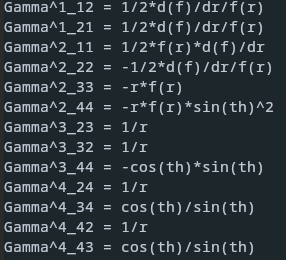
\includegraphics[width=0.35\linewidth]{output_chris.png}
\end{figure}

\hfill 

\hfill 

\hfill 

\textbf{c) } 

\hfill 

\textbf{i)} Utilizando \textit{SageManifolds}, definimos la metrica:
\begin{minted}{python}
# Definir la variedad
M = Manifold(4, 'R^4', start_index=1)
# Definir las coordenadas
c_spher.<t,r,th,ph> = M.chart(r't:(0,+oo) r:(0,+oo) th:(0,pi):\theta ph:(0,2*pi):\phi')
# Definir la función a(t)
f = function('f')(r)

# Definir la métrica g de FRW
g = M.metric('g')
g[1,1] = -f
g[2,2] = 1/f
g[3,3] = r^2
g[4,4] = r^2 * sin(th)^2
#inversa de la metrica 
ginv = g.inverse()
\end{minted}

\hfill 

\hfill 

\hfill

Calculamos el tensor de Riemann con $ R_{\rho\sigma\mu\nu} = \partial_\mu \Gamma_{\rho\nu\sigma} - \partial_\nu \Gamma_{\rho\mu\sigma} + \Gamma_{\rho\mu\lambda} \Gamma_{\lambda\nu\sigma} - \Gamma_{\rho\nu\lambda} \Gamma_{\lambda\mu\sigma} $

\begin{minted}{python}
riem = g.riemann()
print(riem.display_comp(c_spher.frame(), c_spher, only_nonredundant=True))
\end{minted}
\begin{figure}[H]
    \centering
    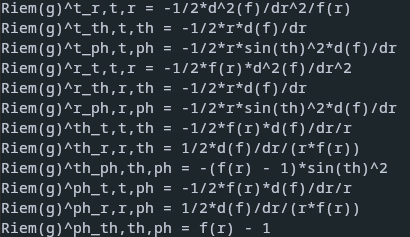
\includegraphics[width=0.35\linewidth]{rieman_metodo1.png}
\end{figure}

\hfill 

\hfill 

\hfill

Calculamos el tensor de Riemann con $ R _{\mu\nu} = g _{\rho\sigma} R _{\sigma\mu\nu}^\rho  $
\begin{minted}{python}
ricci = riem["^s_msn"]
print(ricci.display())
\end{minted}
Resultado: 
\begin{gather*}
  R_{mn} = \left(\begin{array}{rrrr}
  \frac{r f\left(r\right) \frac{\partial^2\,f}{\partial r ^ 2} + 2 \, f\left(r\right) \frac{\partial\,f}{\partial r}}{2 \, r} & 0 & 0 & 0 \\
  0 & -\frac{r \frac{\partial^2\,f}{\partial r ^ 2} + 2 \, \frac{\partial\,f}{\partial r}}{2 \, r f\left(r\right)} & 0 & 0 \\
  0 & 0 & -r \frac{\partial\,f}{\partial r} - f\left(r\right) + 1 & 0 \\
  0 & 0 & 0 & -{\left(r \frac{\partial\,f}{\partial r} + f\left(r\right) - 1\right)} \sin\left({\theta}\right)^{2}
  \end{array}\right) 
\end{gather*}

\hfill 

\hfill 

\hfill 

Calculamos el tensor de Riemann con $ R _{\mu\nu} = g _{\rho\sigma} R _{\sigma\mu\nu}^\rho  $
\begin{minted}{python}
ricciinv = ginv["^mr"]*(ginv["^ns"]*ricci["_rs"])["_r^n"]
ricci_scalar = g["_mn"]*ricciinv["^mn"]
print(f'R = {latex(ricci_scalar.display())}')
\end{minted}
Resultado: 
\begin{gather*}
R = \begin{array}{llcl} & R^4 & \longrightarrow & \mathbb{R} \\ & \left(t, r, {\theta}, {\phi}\right) & \longmapsto & -\frac{r^{2} \frac{\partial^2\,f}{\partial r ^ 2} + 4 \, r \frac{\partial\,f}{\partial r} + 2 \, f\left(r\right) - 2}{r^{2}} \end{array}
\end{gather*}

\hfill 

\hfill 

\hfill 

\textbf{d) }
Supongamos que la ecuación de Einstein tiene una solución como en el Problema (b). Encontrar \( f(r) \).

Partimos de la métrica dada en el problema 3.3.b:

\[ ds^2 = -f(r) \, dt^2 + \frac{1}{f(r)} \, dr^2 + r^2 \left( d\theta^2 + \sin^2\theta \, d\varphi^2 \right) \]

Las componentes de la métrica son:

\[
g_{\mu\nu} = \begin{pmatrix}
-f(r) & 0 & 0 & 0 \\
0 & \frac{1}{f(r)} & 0 & 0 \\
0 & 0 & r^2 & 0 \\
0 & 0 & 0 & r^2 \sin^2 \theta
\end{pmatrix} \qquad \qquad 
g^{\mu\nu} = \begin{pmatrix}
-\frac{1}{f(r)} & 0 & 0 & 0 \\
0 & f(r) & 0 & 0 \\
0 & 0 & \frac{1}{r^2} & 0 \\
0 & 0 & 0 & \frac{1}{r^2 \sin^2 \theta}
\end{pmatrix}
\]

Simbolos de Christoffel:

\begin{gather*}
\Gamma^t_{tr} = \frac{f'(r)}{2f(r)}, \qquad
\Gamma^r_{tt} = \frac{f(r) f'(r)}{2}, \qquad
\Gamma^r_{rr} = -\frac{f'(r)}{2f(r)}, \qquad
\Gamma^r_{\theta\theta} = -r f(r), \\
\Gamma^r_{\varphi\varphi} = -r f(r) \sin^2 \theta, \qquad
\Gamma^\theta_{r\theta} = \frac{1}{r}, \qquad
\Gamma^\varphi_{r\varphi} = \frac{1}{r}, \qquad
\Gamma^\varphi_{\theta\varphi} = \cot \theta
\end{gather*}

A continuación, utilizamos los símbolos de Christoffel para calcular el tensor de Ricci \( R_{\mu\nu} \):

\[
R_{\mu\nu} = \partial_\lambda \Gamma^\lambda_{\mu\nu} - \partial_\nu \Gamma^\lambda_{\mu\lambda} + \Gamma^\lambda_{\mu\nu} \Gamma^\sigma_{\lambda\sigma} - \Gamma^\lambda_{\mu\sigma} \Gamma^\sigma_{\nu\lambda}
\]

Calculamos algunas de las componentes no nulas de \( R_{\mu\nu} \):

\[
\begin{aligned}
R_{tt} &= -\frac{f''(r)}{2} + \frac{f'(r)^2}{4f(r)} + \frac{f'(r)}{r}, \\
R_{rr} &= \frac{f''(r)}{2f(r)} - \frac{f'(r)^2}{4f(r)^2} - \frac{f'(r)}{r f(r)}, \\
R_{\theta\theta} &= 1 - \frac{r f'(r)}{2} - f(r), \\
R_{\varphi\varphi} &= \left( 1 - \frac{r f'(r)}{2} - f(r) \right) \sin^2 \theta
\end{aligned}
\]

La ecuación de Einstein es:

\[
R_{\mu\nu} - \frac{1}{2} g_{\mu\nu} R + \Lambda g_{\mu\nu} = 0
\]

Calculamos el escalar de curvatura \( R \):

\[
R = g^{\mu\nu} R_{\mu\nu}
\]

Después de hacer los cálculos correspondientes:

\[
R = -f''(r) - \frac{4 f'(r)}{r} - \frac{2 (1 - f(r))}{r^2}
\]

Sustituimos \( R \) en la ecuación de Einstein y resolvemos para \( f(r) \):

\[
R_{tt} = -\frac{f''(r)}{2} + \frac{f'(r)^2}{4f(r)} + \frac{f'(r)}{r} = \frac{1}{2} f(r) R - \Lambda f(r)
\]

Reorganizamos esta ecuación para resolver la ecuación diferencial para \( f(r) \):

\[
R_{tt} = -\frac{f''(r)}{2} + \frac{f'(r)^2}{4f(r)} + \frac{f'(r)}{r}
\]

\[
\frac{1}{2} f(r) R = -\frac{1}{2} f(r) \left( f''(r) + \frac{4 f'(r)}{r} + \frac{2 (1 - f(r))}{r^2} \right)
\]

Comparando ambos lados de la ecuación, y simplificando:

\[
-\frac{f''(r)}{2} + \frac{f'(r)^2}{4f(r)} + \frac{f'(r)}{r} = \frac{1}{2} f(r) \left( -f''(r) - \frac{4 f'(r)}{r} - \frac{2 (1 - f(r))}{r^2} \right) - \Lambda f(r)
\]

Desarrollamos y simplificamos:

\[
-\frac{f''(r)}{2} + \frac{f'(r)^2}{4f(r)} + \frac{f'(r)}{r} = -\frac{1}{2} f(r) f''(r) - 2 \frac{f(r) f'(r)}{r} - \frac{1}{r^2} f(r) (1 - f(r)) - \Lambda f(r)
\]

A través de la comparación de términos, observamos que la forma particular de \( f(r) \) que satisface la ecuación es:

\[
f(r) = 1 - \frac{2GM}{r} - \frac{\Lambda r^2}{3}
\]

\end{document}
